%
\documentclass{article}
\newcommand{\assgnnum}{5}
\newcommand{\assigndate}{January 24}

\usepackage{amsmath}
%\usepackage{fullpage}
\usepackage{amssymb}
%\usepackage{bbm}
\usepackage{fancyhdr}
%\usepackage{paralist}
\usepackage{graphicx}
\usepackage[pdftex,colorlinks=true, urlcolor = blue]{hyperref}
\usepackage{../../arbenson-math}

\oddsidemargin 0in \evensidemargin 0in
\topmargin -0.5in \headheight 0.25in \headsep 0.25in
\textwidth 6.5in \textheight 9in
\parskip 6pt \parindent 0in \footskip 20pt

% set the header up
\fancyhead{}
\fancyhead[L]{CME193: In-class exercises \assgnnum}
\fancyhead[R]{\assigndate}
%%%%%%%%%%%%%%%%%%%%%%%%%%
\renewcommand\headrulewidth{0.4pt}
\setlength\headheight{15pt}


\newcommand{\p}{\ensuremath{\mathbf{P}}}
\renewcommand{\Pr}[1]{\ensuremath{\p \left \{ #1 \right \}}}
\newcommand{\nti}{\ensuremath{n \to \infty}}
\newcommand{\I}{\ensuremath{\operatorname{I}}}
\newcommand{\One}[1]{\ensuremath{\mathbbm{1}_{\left \{ #1 \right \}}}}
\newcommand{\E}{\ensuremath{\mathbf{E}}}
\newcommand{\Ex}[2][]{\ensuremath{\E_{#1} \left[ #2 \right]}}
\newcommand{\var}{\ensuremath{\operatorname{Var}}}
\newcommand{\cov}{\ensuremath{\operatorname{Cov}}}
\newcommand{\F}{\ensuremath{\mathcal{F}}}
\newcommand{\R}{\ensuremath{\mathbb{R}}}
\newcommand{\C}{\ensuremath{\mathbb{C}}}
\newcommand{\NormRV}[2]{\ensuremath{\operatorname{N}\left(#1, #2\right)}}
\newcommand{\BetaRV}[2]{\ensuremath{\operatorname{Beta}\left(#1, #2\right)}}
\newcommand{\argmax}{\operatornamewithlimits{argmax}}
\newcommand{\x}{\mathbf{x}}
\newcommand{\A}{\mathbf{A}}
\newcommand{\bb}{\mathbf{b}}


\newcounter{points}
\setcounter{points}{0}

\newcommand\setpoints[1]{\addtocounter{points}{#1}(#1 points)}
\newcommand\printpoints{Total number of points: \thepoints}

\newcommand{\eqD}{\ensuremath{\overset{\mathcal{D}}{=}}}

\setlength{\parindent}{0in}

\begin{document}

\pagestyle{fancy}
%\vspace*{15pt}
\begin{enumerate}

\item \textbf{KDE Plot}

Recall the definition of a KDE: given a sample $x_1, x_2, \dots, x_n$ from an unknown distribution $f$ the kernel density estimate of $f$ at point $x$ with kernel $K_b$ is defined as 
$$\hat{f}(x;b) = \frac{1}{n}\sum_{i=1}^{n}K_b(x-x_i)$$
where the kernel must satisfy $\int_{-\infty}^{\infty}K(u)du = 1$ and $K(-u) = K(u).$ The parameter $b$ is known as the bandwidth and controls the width of the kernel used. 
\begin{enumerate}
\item generate data from the exponential distribution with scale 1 
\item write a function that computes a KDE with a Gaussian kernel. Here the bandwidth refers to the standard deviation of the Gaussian kernel.
\item plot both the data you generated as X's and the KDE as a line plot on the same axis
\end{enumerate}







\item \textbf{Recreate the Images Below}

hint: \texttt{plt.scatter}
\begin{figure}[h]
\centering
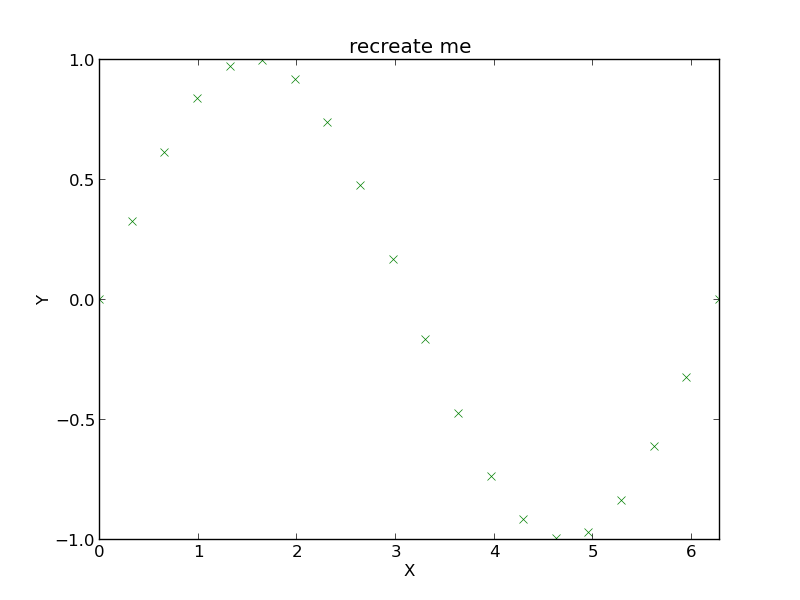
\includegraphics[width=.5\textwidth]{images/recreate_plot.png}
\end{figure}

\begin{figure}[h]
\centering
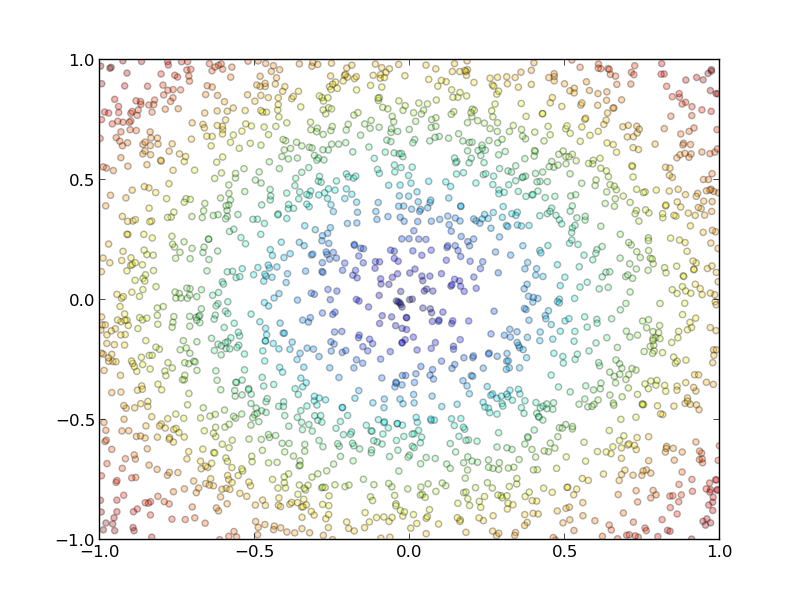
\includegraphics[width=.5\textwidth]{images/rainbow_plot.png}
\end{figure}


\end{enumerate}
\end{document} 
